\section{Introduction}
Today, mobile devices run third party applications to perform complex tasks like web browsing, banking and gaming. Recent studies have found that smart-phones are the target of an increasing number of malware attacks \cite{bose2006mobile, cybercriminals2007banks, iphone2010seriot} and their security is important as personal data such as contacts, credit card numbers and passwords are often stored on the device. While some security models \cite{androidsecurity} provide a stronger process level isolation among applications, operating system bugs such as \cite{sms2009iphone,opencore2009android,kernel2009vulnerability} allow malicious applications to take over the device. Recent reports have even found that some smart phones had the Mariposa botnet pre-installed \cite{mariposa2009android}. Virtualization can be useful for secure isolation of third party code from confidential data and provide greater defense-in-depth against attacks on the system.\\

In recent years, virtual machines have become prevalent in cluster computing environments \cite{gartner2009virtual} as they provide isolation for shared usage of machines in a data center. As a result of hardware improvements, smart phone configurations found today resemble desktop machines from few years ago and many of them run commodity operating systems. There is a growing interest in academia \cite{cox2007pocket} and industry \cite{vmware2009nextfrontier} about the benefits of virtualization on these devices. Virtualization provides better security guarantees in mobile devices than current solutions offer as well enabling useful applications like environment migration. \\

Migrating a system to a mobile device can take advantage of network or computation facilities that are closer to the user's location and provide the user with a consistent experience irrespective of the network connectivity. Environment migration has been studied earlier, in the context of servers in a cluster \cite{clark2005live} and enables administrators of clusters to perform maintenance tasks without interruption. On the other hand, migration techniques on mobile devices can help maintain consistent snapshots which allow easy transfer of data when users switch mobile phones and to roll-back the system to a previously known state.\\

\begin{figure*}[tbh]
\centering
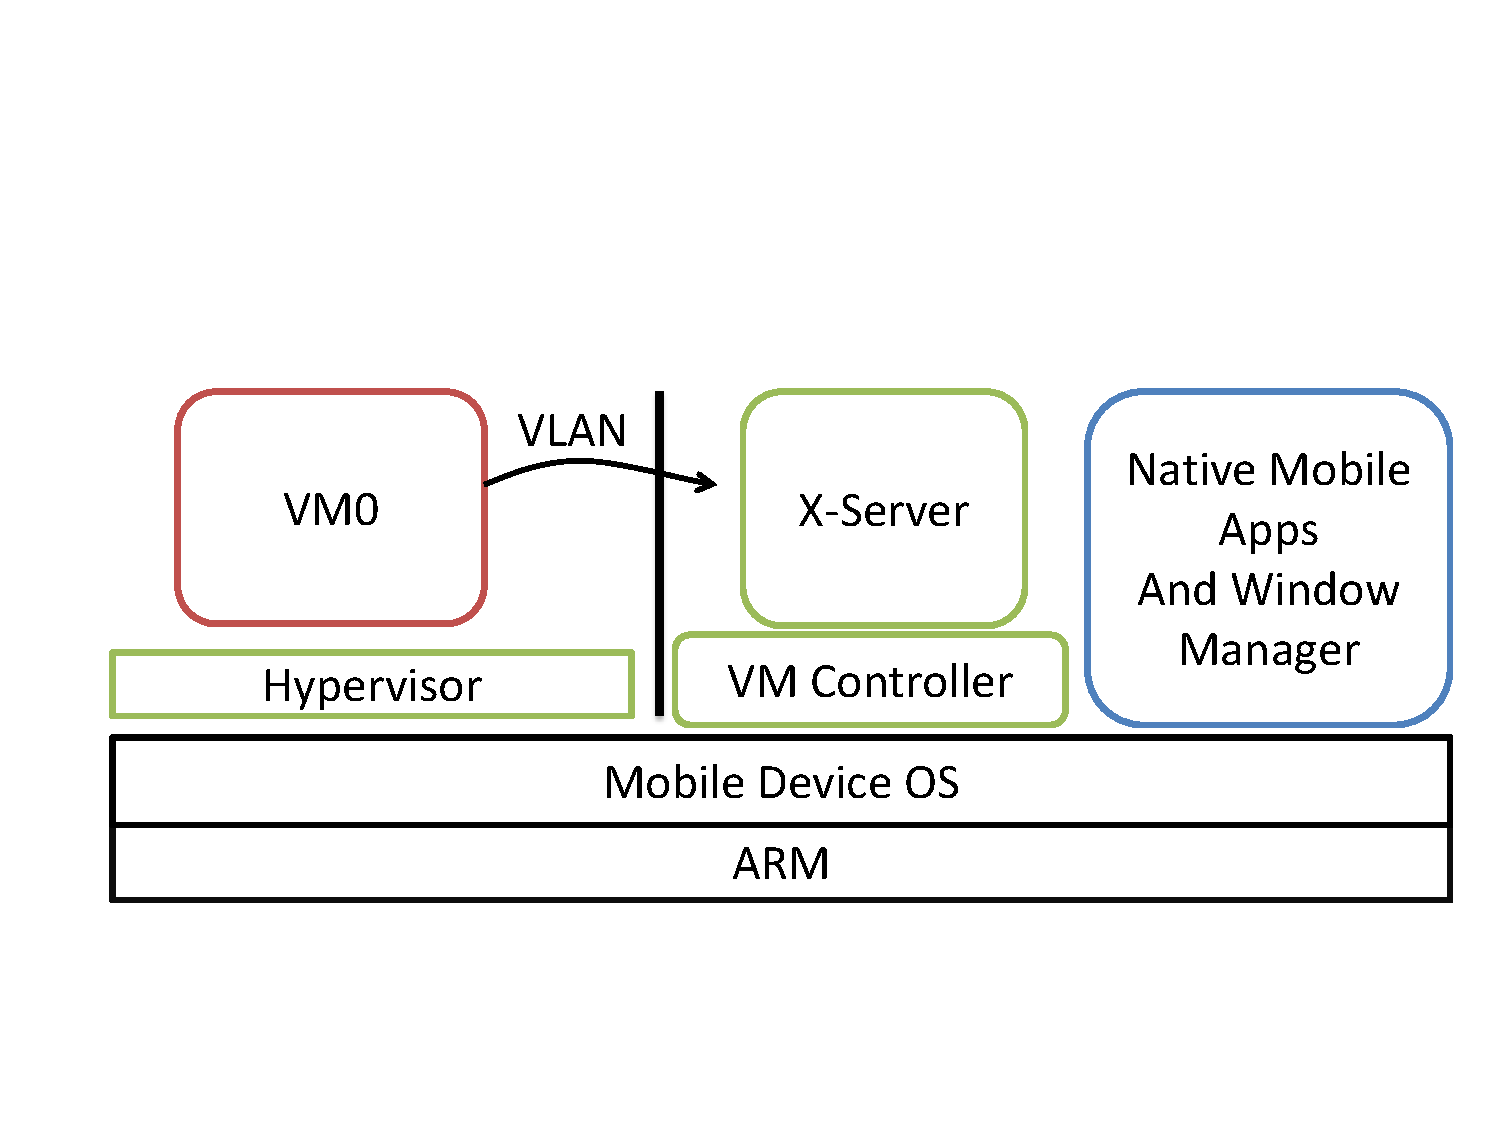
\includegraphics[width=1.5\columnwidth]{arch}
\caption{Architecture diagram}
\label{fig:arch}
\end{figure*}
Existing solutions for isolation of mobile applications introduce a Type I hypervisor \cite{mvp, okl4} which manages the phone's hardware and allows running multiple operating system on top. While these solutions are useful, it would be better to have isolated applications which are integrated with the host operating system's application launcher and does not suffer from a large performance penalty. In order to achieve this goal, we propose to have an isolation framework running on the host operating system and a shared rendering engine for improved performance. Since most of the mobile devices work on the ARM architecture, we plan to evaluate how different virtualization techniques perform on ARM.\\

Our preliminary investigations evaluate the difference in performance between emulating ARM-on-ARM vs x86-on-ARM and our results show that ARM-on-ARM virtualization has much lower performance overhead, however, even ARM-on-ARM is prohibitively slow, and any machine emulation simply is not reasonable on a smartphone.  Given the large overheads of machine emulation, we had to explore alternative means of virtualization.  We looked into Xen and KVM, two popular virtualization solutions for x86, however we discovered that their implementations on ARM simply were nowhere near mature enough for our needs. \\

Next, we explored an OS-level virtualization tool called Linux Containers (LXC). Linux Containers present a low overhead technique of isolating a process within a container.  A container is made up of several namespace virtualization techniques, where the UID, user namespace, network resources and more are virtualized in order to prevent the process inside the container from interfacing external data or resources.  Despite some difficulties in getting Linux Containers to run, it has been very effective.  After extensive testing, it has proved to be an ideal intersection of isolation and performance. \\

We believe that an integrated solution where untrusted applications are integrated with mobile device would enable wider adoption. The rest of this report is structured as follows: Section \ref{sec:design} presents an overview of the design and also describes in detail some of the design choices which we make. Sections \ref{sec:impl} describes the preliminary implementation and deployment of virtualization on two smart phones and also discusses details about porting the X server. Evaluation of our existing system is presented in \ref{sec:eval}. Section \ref{sec:related} discusses existing efforts in this area and section \ref{sec:conclusion} concludes. \\

